
\section{Introduction}
Since the objective of this thesis is to study various alternatives for reducing the energy consumption of software programs, this chapter will focus on this topic. We shall conduct extensive empirical research. This chapter describes the instruments required to conduct a successful experiment to measure the energy consumption of software applications.
In addition, the majority of the time we will conduct an analytical comparison; therefore, the goal is to develop a framework to assist practitioners in comparing various solutions in terms of energy consumption.


First we will project the challenges of benchmarking to the case of energy consumption and see when it deffers from the previous contexts.
then we will propose a framework to deal with those challenges.
later we will elaborate each part of the framework and how to solve certain of these challenges.


A reproducible setup environment needs to be established in order to maximize the software's potential to reduce energy consumption.

This chapter will be devoted to giving a set of guidelines with the intention of delivering a test that is accurate, representative, and replicable.

% This chapter will go over each component in further detail, describe it, and explain how it is used in the field of empirical analysis for software energy optimization.




%%%%%%%%% preliminary taughts and section structure 
% The need of reproducibility in our field - software optimization based on empirical studies -

% The importance of Virtualisation for reproducibility \cite{howe_virtual_2012}
% some of the most important parts are
% - fewer constraints on research methods
% - on-demand backups
% - virtual Machines as Publications
% - more Variables captured



%%%% part of the state of the art 
% In the area covered by this PhD thesis, reproducibility might be achieved by ensuring the same execution settings of physical nodes, virtual machines, clusters or cloud environments.
%%% why it won't work for energy consumption 
% However, when it comes to measuring the energy consumption of a system, applying acknowledged guidelines and carefully repeating the same benchmark can nonetheless lead to different energy footprints not only among homogeneous nodes, but even within a single node.
%% reseasons why 
% One major problem that hinders the reproducibility of the empirical benchmarks is the interaction with the external environment, either as concurrency or dependencies.
% Therefore, researchers cannot observe the same results, unless they duplicate the same environment.


%%% FOR METRICS AND ACCURACY 

%%%% this is relative about my thesis 
In theory, using identical CPU, same memory configuration, similar storage and networking capabilities, should increase the accuracy of physical measurements.
Unfortunately, this is not possible when it comes to measuring the energy consumption of a system.
Applying the benchmarking guidelines and repeating the same experiment with in the same configuration are not sufficient to reproduce the the same energy measurements, not only between identical machines, but even within the same machine.
This difference---also called \emph{energy variation} (EV)---has become a serious threat to the accuracy of experimental evaluations.

Figure~\ref{fig:motivation} illustrates this variation problem as a violin plot of $20$ executions of the benchmark \emph{Conjugate Gradient} (\textsf{CG}) taken from the \emph{NAS Parallel Benchmarks} (NBP) suite~\cite{Bailey:1991:NPB:125826.125925}, on $4$ nodes of an homogeneous cluster (the cluster \textsf{Dahu} described in Table~\ref{table:g5k}) at 50\,\% workload.
We can observe a large variation of the energy consumption, not only among homogeneous nodes, but also at the scale of a single node, reaching up to $25\,\%$ in this example.

\begin{figure}%[!htb]
    \center{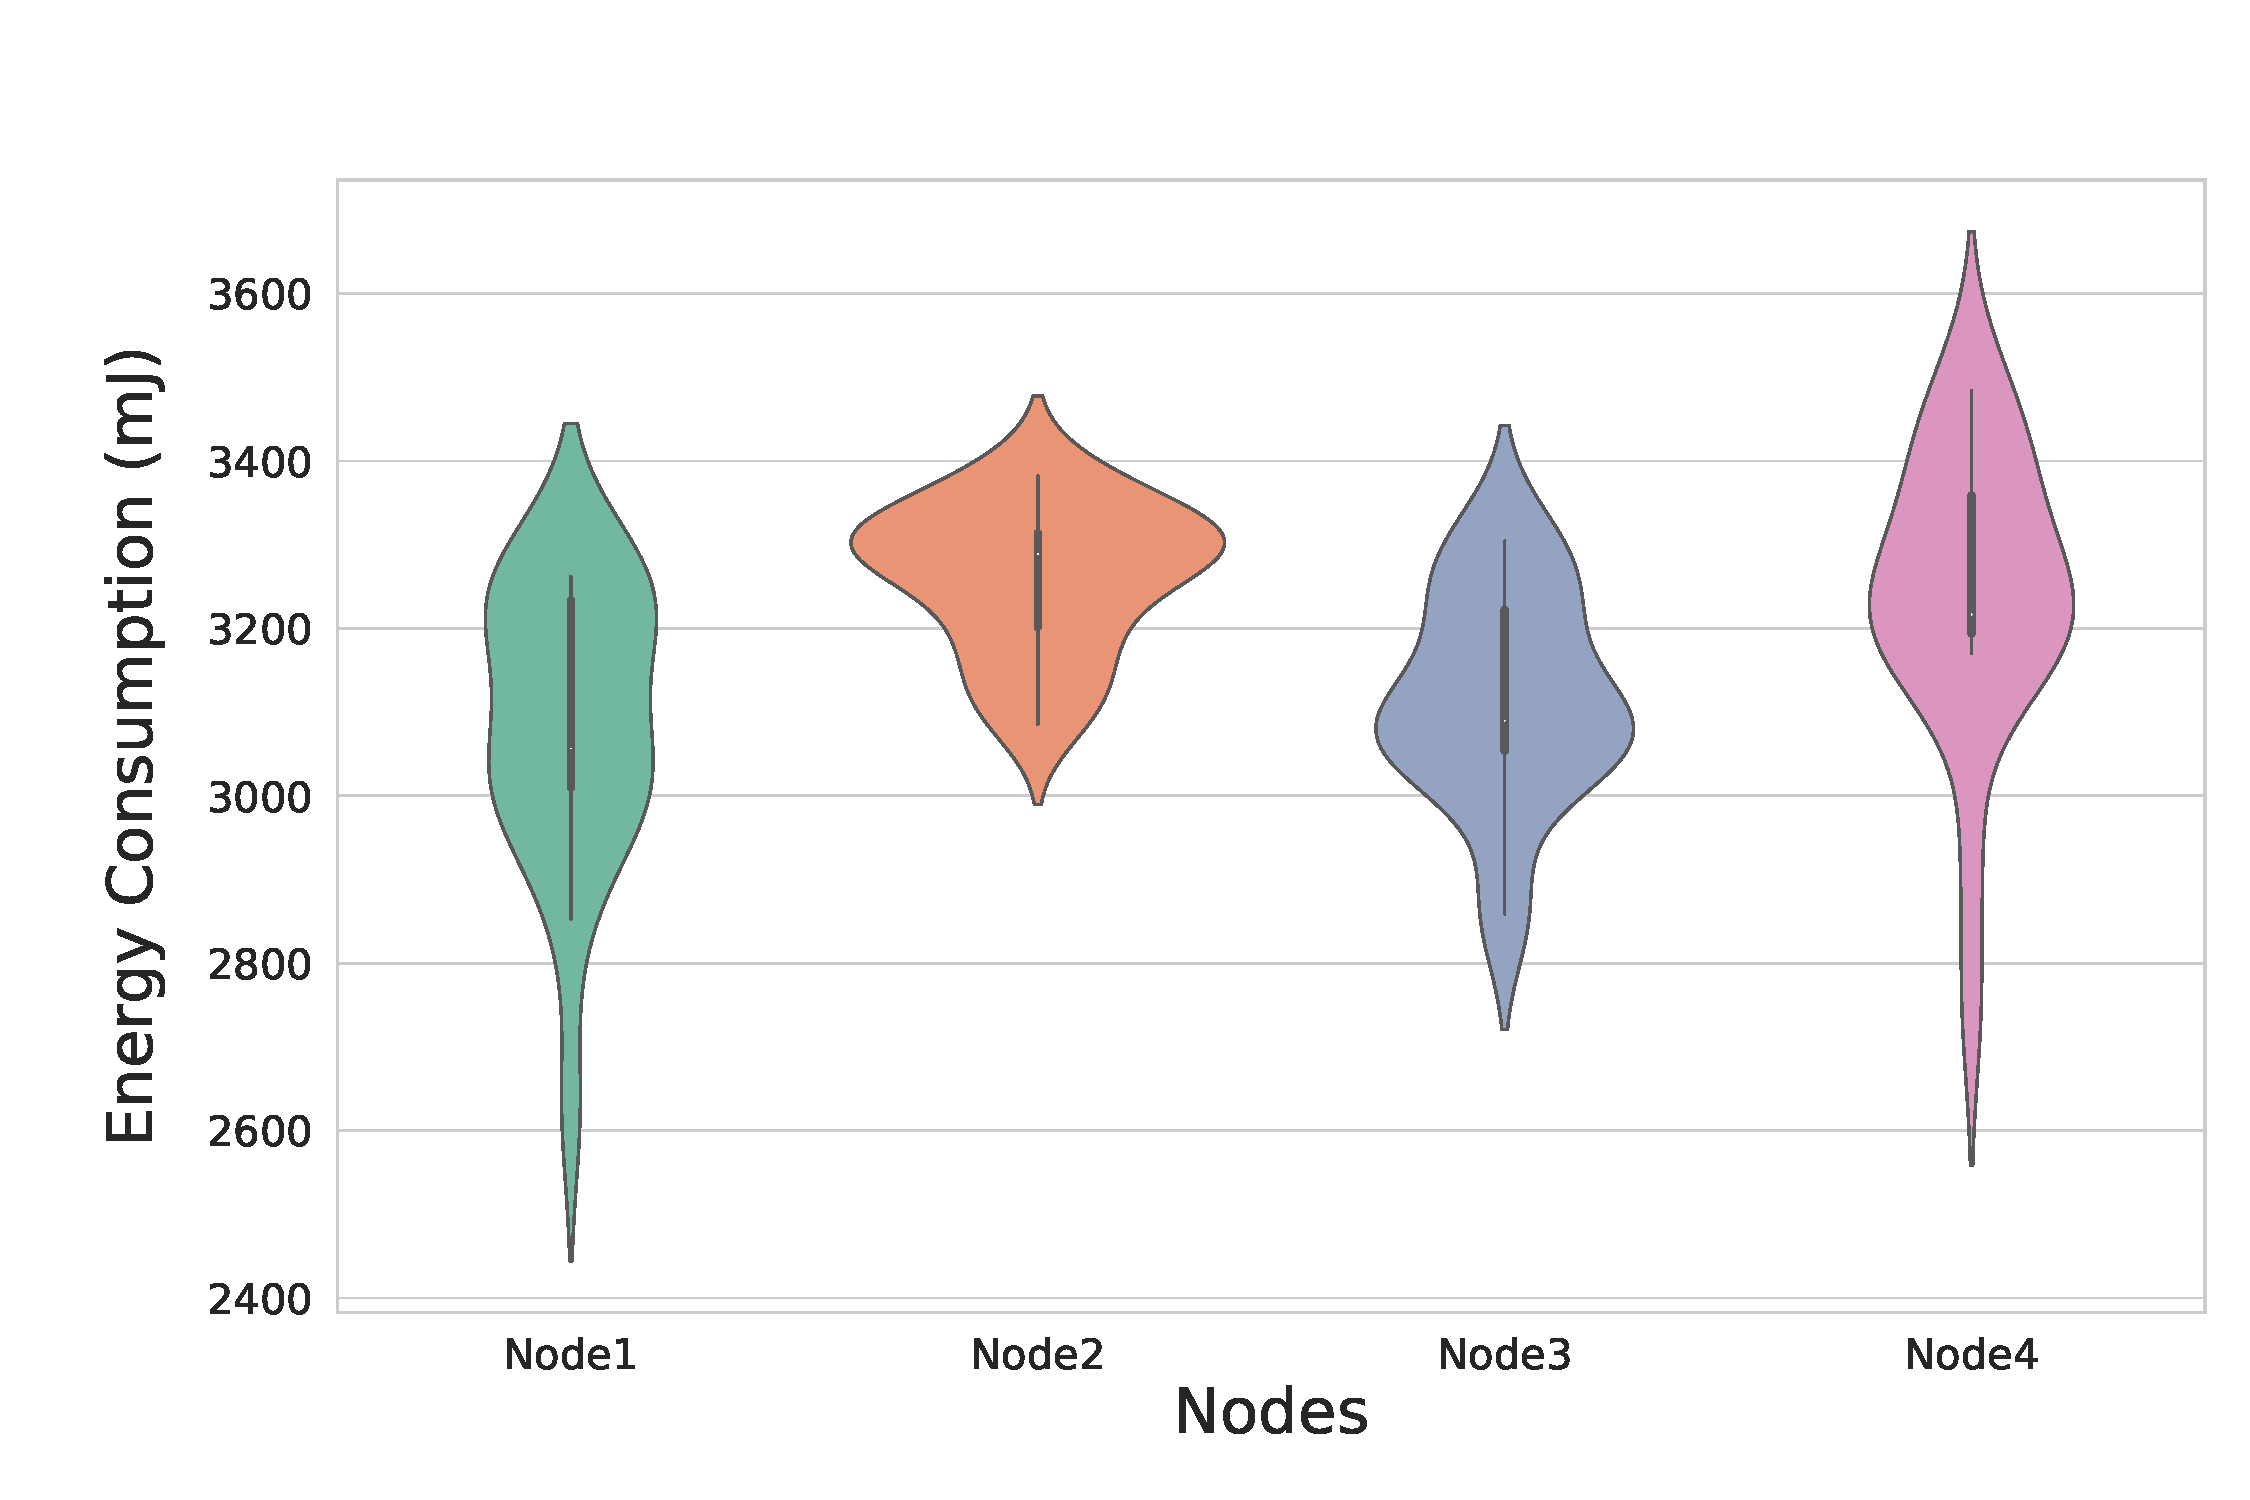
\includegraphics[width=.9\linewidth]{imgs/motivation}}
    \caption{CPU energy variation for the benchmark \textsf{CG}}\label{fig:motivation}
\end{figure}
%% state of the art 
Some researchers started investigating the hardware impact of the energy variation of power consumption.
As an example, one can cite~\cite{borkar_designing_2005,tschanz_adaptive_2002} who reported that the main cause of the variation of the power consumption between different machines is due to the \textbf{CMOS} manufacturing process of transistors in a chip.
\cite{heinrich_predicting} described this variation as a set of parameters, such as CPU Frequency and the thermal effect.



As Stephen M. Blackburn~\emph{et~al.} cited in their paper "evaluate collaboratory"~\cite{stephen_evaluate_2012}, one of the major pitfalls of the measurement contexts is the inconsistency, which can be translated here by the fact that the production context is not the same as the benchmarking one.

Another difficult part for practitioners is to generalize the claims they reached beyond the lab conditions.
Are they appropriate?
Are they consistent and are they reproducible?
To answer those questions, the community agreed on some wellknown benchmarks to represent a specific concern of the production world.
One can site as an example the Dacapo~\cite{DaCapo:paper} and Renaissance~\cite{renaissance} benchmark suites for Java applications, or the CLBG benchmark suite for comparing programming languages\footnote{\url{https://benchmarksgame-team.pages.debian.net/benchmarksgame/index.html}}.
Although they do not cover all the cases, the community agrees on their relevance and representativeness.

In addition to these benchmarks, a new category of testing techniques has emerged to simulate the worst cases of the production environments. This new category of benchmarking called performance tests\cite{pradeep2019pragmatic}, which are benchmarks meant to evaluate the behavior of software under stress situations. We can use the Gatling\footnote{\url{https://gatling.io/}} as an illustration for web applications stresser and stress-ng for hardware heavy workload perormance measurements~\cite{king2017stress}.






%%%% THIS Should the introduction of my chapter 

\subsection{Extension}
Morover, The field of computer science is seeing rapid advancements, which has led to an increase in the number of obsolete results. Even more so, when it comes to studies that compare multiple solutions, it is impossible to cover them all.
In addition, between the preliminary experiment and the results that were published, there may have been the appearance of new candidates as well as the development of others. As a result, we would like to provide a fresh idea for a productive experiment that we will call "Extension." The ability to give the required tools to not only repeat the experiment but also to add additional candidates, workloads, or key metrics.


%% how to extend 

We propose making certain enhancements to the benchmarking framework that was suggested by the collaboratory on Experimental Evaluation of Software \footnote{\url{http://evaluate.inf.usi.ch/}}. and Systems in Computer Science in order to address those problems.
Instead of only presenting the four primary aspects of their guidelines, which are \emph{measurement contexts} that indicate the software and hardware components that will alter or remain constant during the experiment. \emph{workloads} which identify the benchmarks to use in the experiment, as well as their inputs; \emph{metrics} that specify the attributes to be measured and how to assess them. \emph{Data analysis} show how to examine data and evaluate the outcomes of the analysis to offer insight into the assertions that arise from the study.

\begin{itemize}
    \item \textbf{candidates}: a set of candidates that will be used in the experiment. The candidates should be agnostic of the experiment context and they all
\end{itemize}





\begin{figure}%[!htb]
    \center{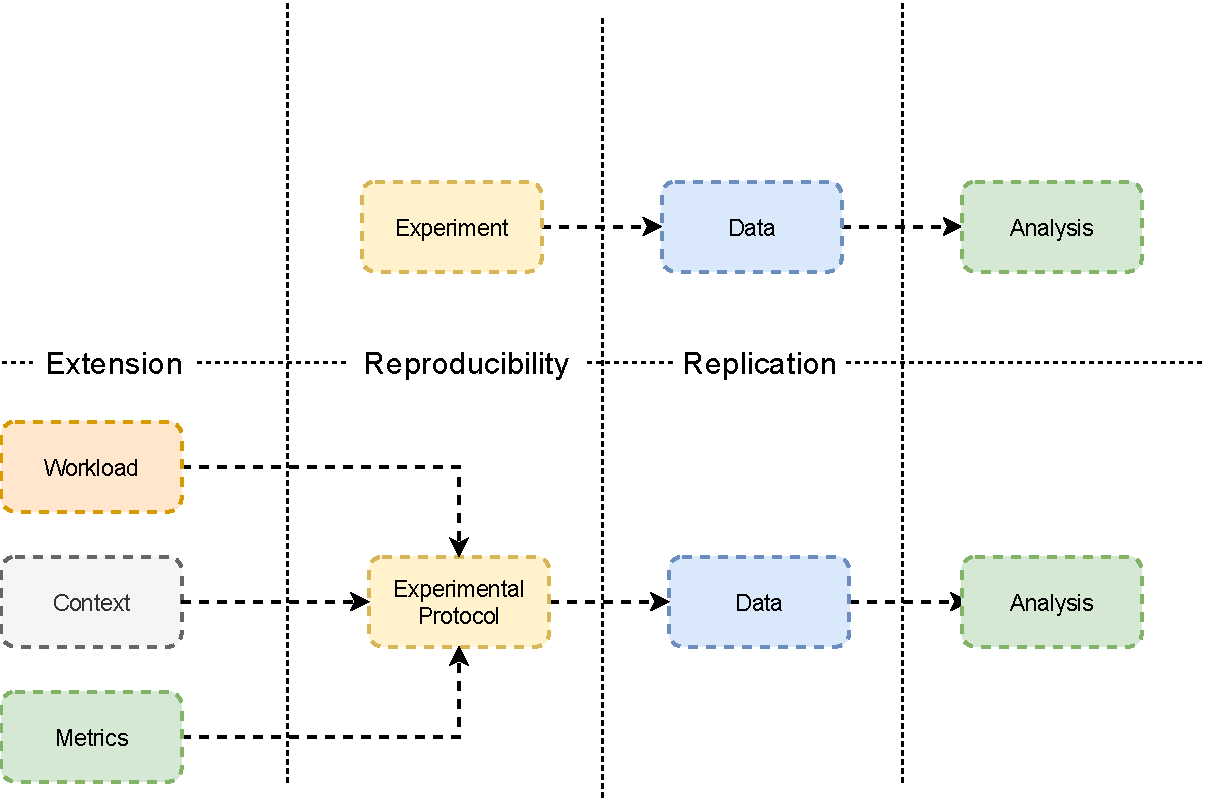
\includegraphics[width=.9\linewidth]{imgs/benchmarkingprotocol}}
    \caption{Benchmarking protocol}\label{fig:benchmarkingprotocol}
\end{figure}



% A more subtle issue may arise due to the values of the measurements that we achieved.
% In fact, the energy measures are quite small, and iterations may be taking a few milliseconds more or less to run.
% A thing we cannot measure using our measurement tools.
% How generalizable are our results? As a set of energy variation optimization guidelines, we argue that our results applied on most of the modern Intel CPU.
% However, using and comparing identical CPU is still tricky and is very dependent to chips.


\section{Reproducibility in benchmarking }


%% just a placeholder title for the moment 
% introduction of vms 


\subsection{Virtual machines}
To resolve this problem, practitioners tend to use Virtualisation. Using virtual machines aka VM gives reaserchers the freedom to choose their own tools, software and operating system that they are the most confortable with without paying the price to change the actual working environment, which will give them eventually more controle over the dependencies and the execution environement. Moreover, using a vm will solve the \emph{replication crisis} thanks to the virtual images, even the most complex architecture can be reproduced easily by just instantiating a copy of the image. Since the virtual machines are agnostic to the host architecture, reaserchers won't have to worry about where and how their experiments are replicated because they have already setup the execution environement. Another advantage to the virtual machines is the snapshot mechanism, it allows reaserchers to create backups and revert some changes with simple clicks. Last but not least,thanks to the isolation, virtual machines push the reproducibility further by allowing the future usages to see all the variables -controled and uncontroled-  and do other analysis without dealing with any dependencies. In his paper \cite{howe_virtual_2012} bill howe lists the advantages of using virtual machines in reaserchers experements including the economical impact and cultural limitation to a such approach.

which allow them to have control over the ressouces, the dependencies and the execution environment. Moreover, thanks to the snapshots, deploying a software is easily done by instantiating a copy of that image.
However, this choice comes with a certain cost. Because the intervention of the hypervisor,the software will use two kernels , the virtual machine one and the host machine one, which will provide a noticiable overhead, and will impact the performances of the tests.Therefore, we can't use virtual machines for exepements that are related to performance. Another limiation with the virtual machine is the the isolation. It is true that this feature will prevent the experience environement with any undesirable interference from the outside world. but sometimes this contact is needed, especially when the experiment is dependent to an external part, such as sensors. In energicial tests we tend to use hardware powermeters which will make it difficult to use the virtual machines in this case .

% introduction of docker 

\begin{figure}
    \center{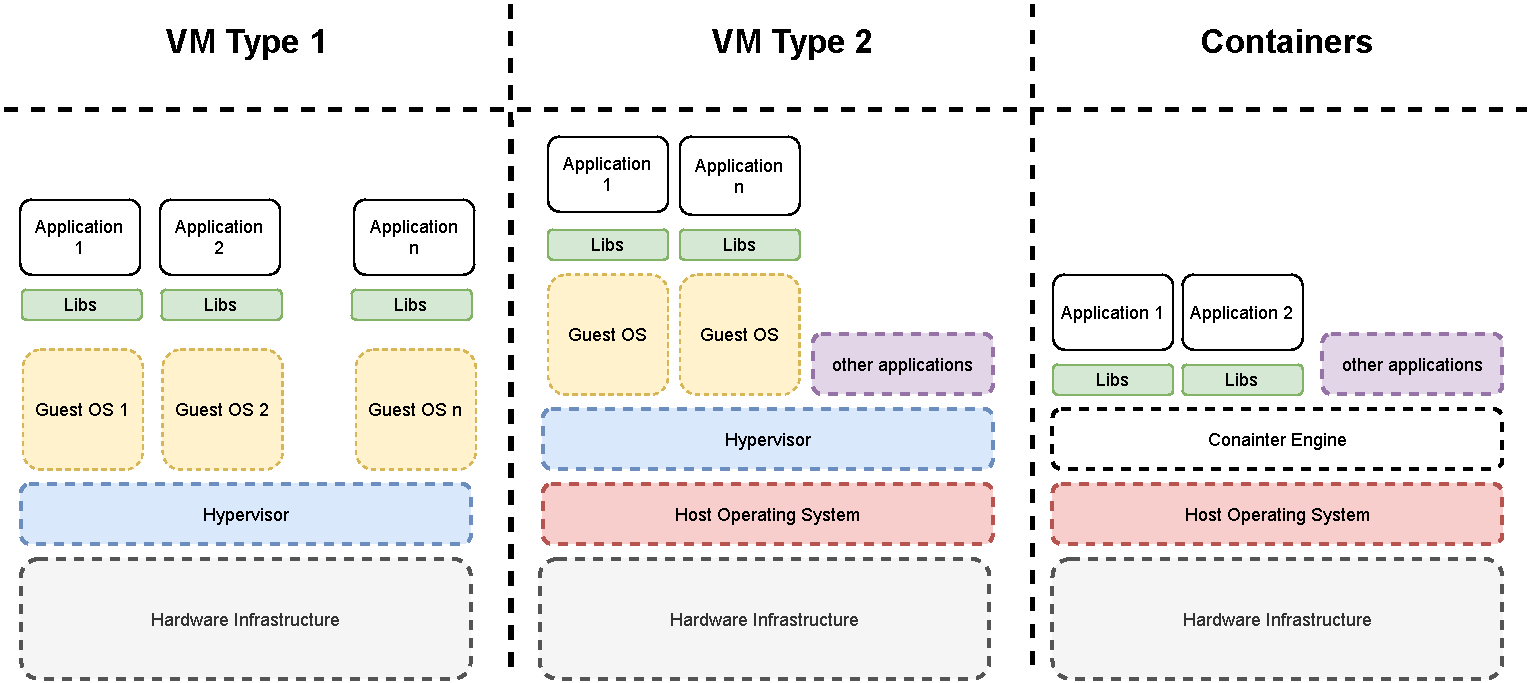
\includegraphics[width=1\linewidth]{imgs/virtualization_techniques}}
    \caption{Different Methods of Virtualzation}\label{environement:virtualization_technique}
\end{figure}

\subsection{Containers}

another solution would be using something that allows us to have the isolation from the host os and the ease of replication that virtual machines offer, and the direct interaction with the hardware that the classical method give.
contarization offers a such advantages while keeping the isolation and the ease of replication for application.

Figure \ref{environement:virtualization_technique} explains the differents in architecture between the clasic types2 of Virtualisation and Containers.
\begin{itemize}
    \item Type 1: runs directly on the hardware, it is mainly used by the cloud providers where there is no main OS, but just virtaul machines, we can site for this the open-srouce XEN and VMware ESX
    \item Type 2: runs over the hostmachine Operating System, mostly used for personal comptuers, VMware server and virtualBox are famous examples of this type, most of the reaserchers expermentation are run witht this type, howerver due to the 2 Operatings syestms the applications tend to be more slower
    \item containers : Instead of its own kernel, containers used the hots kernel to run their Os, which makes them ligher, quickers and use the full pontial use of the hardware. For this we can cite \emph{Docker}, \emph{Linux LXC}\emph{LXD} \cite{abuabdo_virtualization_2019}
\end{itemize}
%  TODO Rephrase so i include it before VMs+ add links to the technologie


\subsection{Docker vs Virtual Machine}
Depsite that Type 1 is more performant than type 2, the second one is the most used in reaserch, since most researchers conducts their experements in their own machine. In the other hand, docker is the most famous thechonology for for containers.
In ower case we are more prone to docker for two reasons.
\begin{enumerate}
    \item we need a litetweight orchestrator to not affect the energy consumption of ower tests. As prior work mentioned [cite Morabito (2015) and van Kessel et al. (2016)]
          % cite Power efficiency of hypervisor-based virtuali- zation versus container-based virtualization. University of Amsterdam.
    \item since we are using the hardware itself to measure the energy consumption, we are required to interract with the host OS itself.
\end{enumerate}
Special notice to \href{https://github.com/powerapi-ng/virtualwatts}{virtualwatts}. A framework that allows us to retireve the energy consumption of a virtual machine.
%%%%% THINGS TO ADD : 
%% -------------- Dont think so 
% the impact of docker on the reprodudicibility 
% Limits of docker 
% The docker files and the clarification of the methodology 
\subsection{Docker and energy}
Now that we have chosen to go with the containers technorolgy to encapsulate our tests. What would be the impact of this solution on the energy consumption of our tests.

Based on the studies of \cite{santos2018does}, who analysed the impact of adding the docker layer on the energy consumption.
In their experement. Eddie Antonio et al run multiple benchmarks with and without docker. and compared their energy consumption and execution time.
The first step was to see the impact of docker deamon while there is no work. to see the impact of the orchestrator alone. Later they had the experiment with the following benchmarks
\begin{itemize}
    \item wordpress
    \item reddis
    \item postfresSQL
\end{itemize}
The following figures represents the energy consumption of the system while it is idle. As we can see  in figure \ref{fig:docker_idle} Docker braught arround 1000joules overhead.
\begin{figure}
    \center{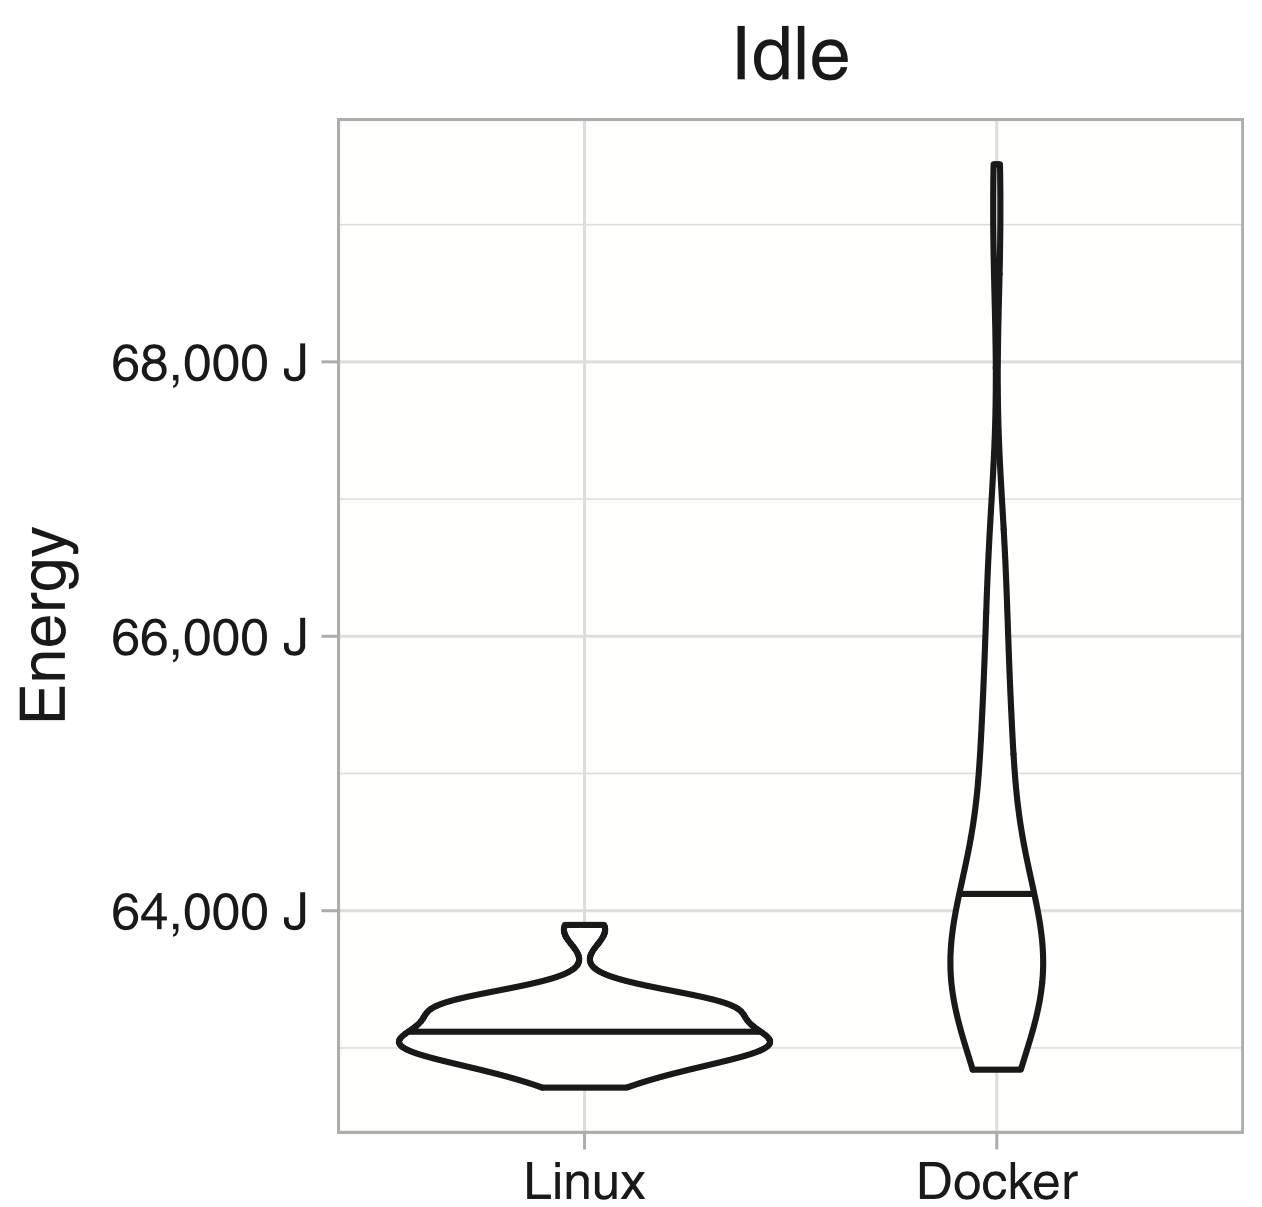
\includegraphics[width=.5\linewidth]{imgs/docker_vs_vm_energy_paper/idle_energy}}
    \caption{energy consumption of Idle system with and without docker \cite{santos2018does}}\label{fig:docker_idle}
\end{figure}
In the other hand as we can see in figure \ref{fig:docker_reddis}. docker increased the execution time of the benchmark by 50 seconds which caused an increase in energy since they are highly correlated.
The authors also highlated the fact that this increase of energy consumption is due to the docker deamon and not the fact that the application is in a container. Moreover they estimted the price of this extra energy and it was less than 0.15\$ in the worst case. Which is non significant compared to the advantages that docker bring for isolation and reproducibility.\\
if we  recap this study in one sentence,it would be the following one.
The dockerised softwares tend to consume more energy, because mainly they take more time to be executed.
The average power consumption is higher with only \textbf{2Watts} and it is due to the docker deamon.This overhead can be up to 5\% for IO intensive application, but it is mearly noticiable when it comes to CPU or DRMA intesive works



\begin{figure}
    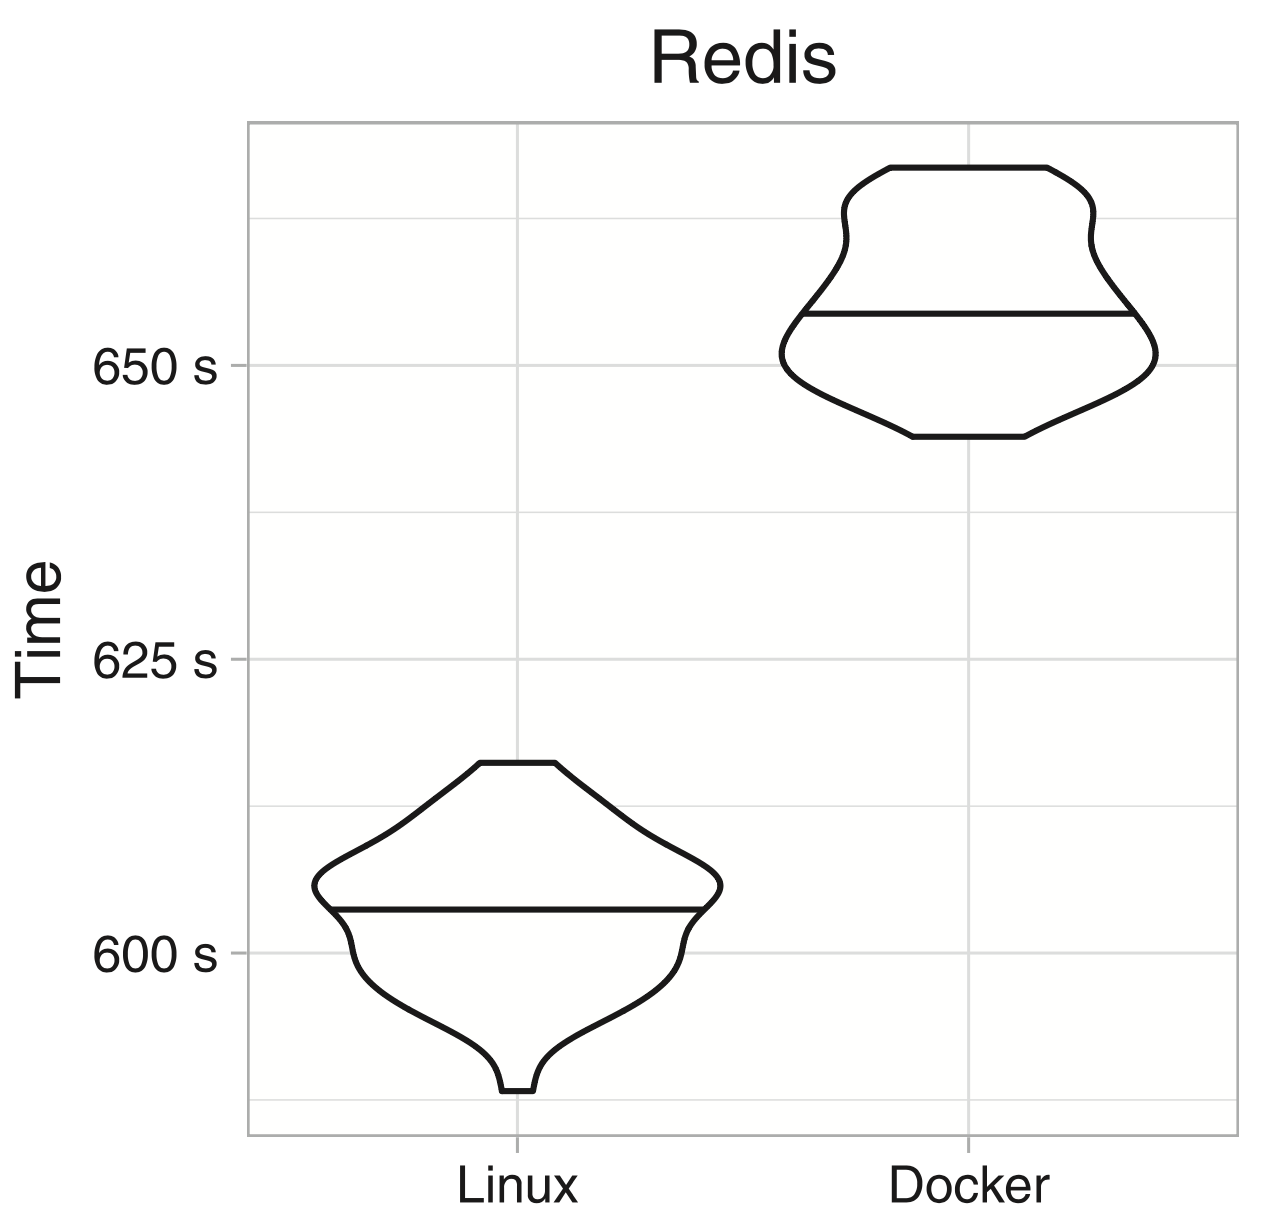
\includegraphics[width=.5\linewidth]{imgs/docker_vs_vm_energy_paper/reddis_time}
    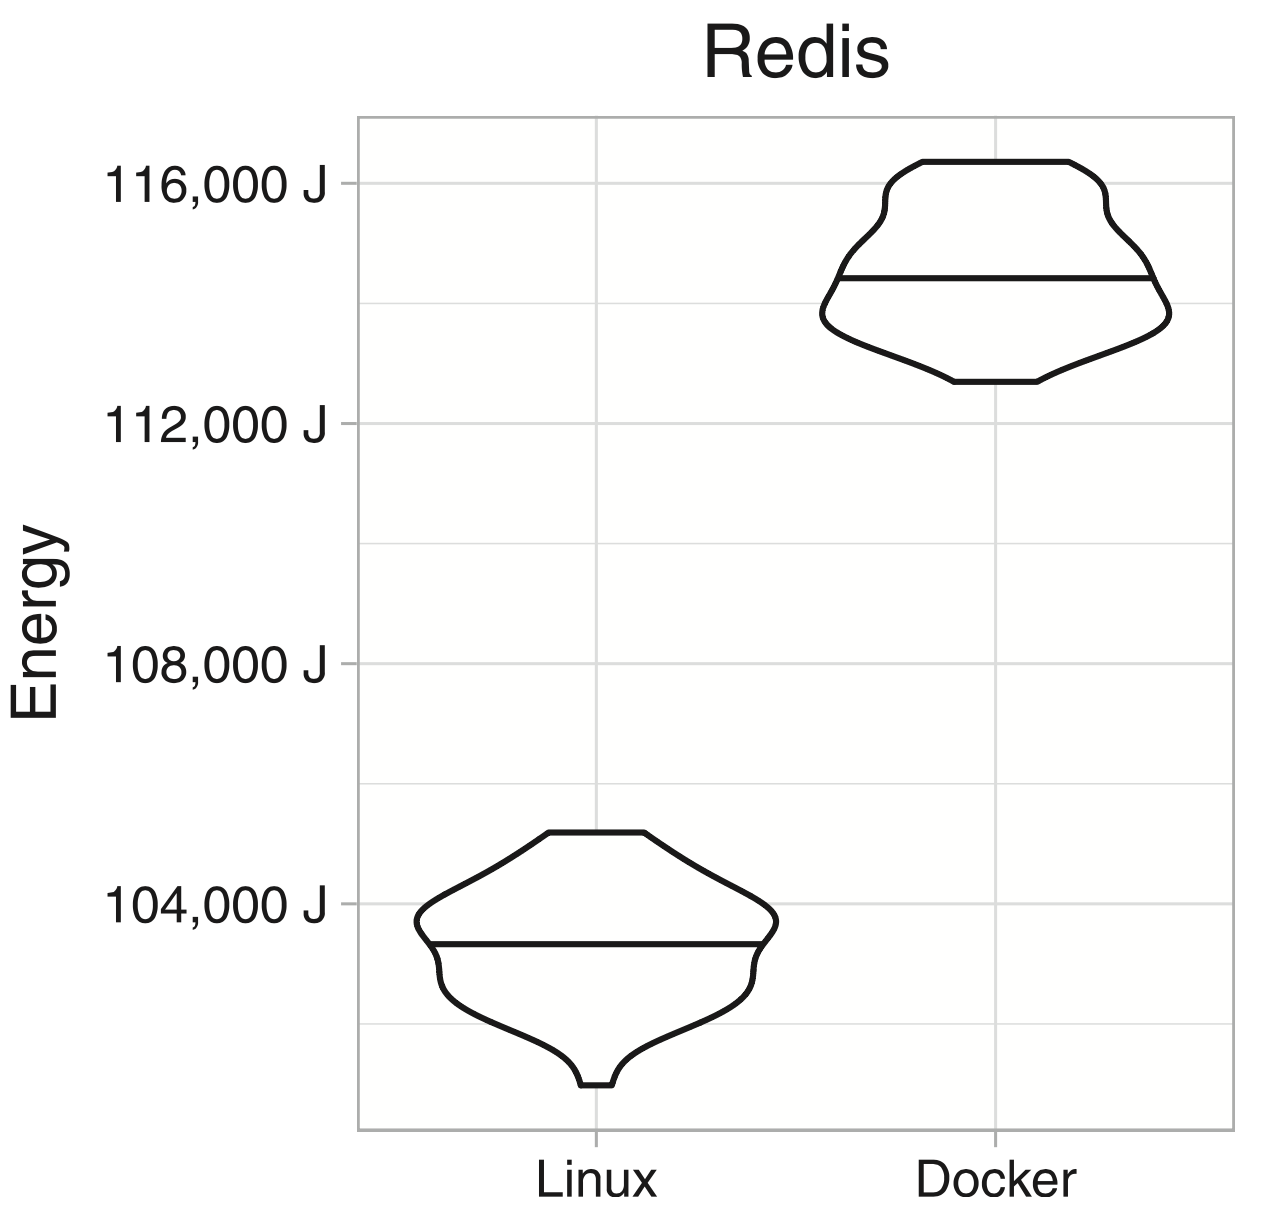
\includegraphics[width=.5\linewidth]{imgs/docker_vs_vm_energy_paper/reddis_energy}
    \caption{execution time and energy consumption of Redis  with and without docker \cite{santos2018does}}\label{fig:docker_reddis}
\end{figure}


\subsection{docker and accuracy}
And now Since the stat of the art has aggreed on the impact of docker on the energy consumption,Let's discuss it's impact on the accuracy. In other words\\
\textbf{RQ :} does Docker affect the energy variation of the exepements ?

To Answer this question we have conducted a preliminary experiment by running the same benchmarks \textsf{LU}, \textsf{CG} and \textsf{EP} in a Docker container and a flat binary format on 3 nodes of the cluster \textsf{Dahu} to assess if Docker induces an additional variation.
Figure~\ref{fig:docker} reports that this is not the case, as the energy consumption variation does not get noticeably affected by Docker while running a same compiled version of the benchmarks at 5\,\%, 50\,\% and 100\,\% workloads.
In fact, while Docker increases the energy consumption due to the extra layer it implements~\cite{eddie_antonio_santos_how}, it does not noticeably affect the energy variation.
The \emph{standard deviation} (STD) is even slightly smaller ($STD_{Docker}=192 mJ$,$STD_{Binary}=207 mJ$), taking into account the measurements errors and the OS activity.

\begin{figure}
    \center{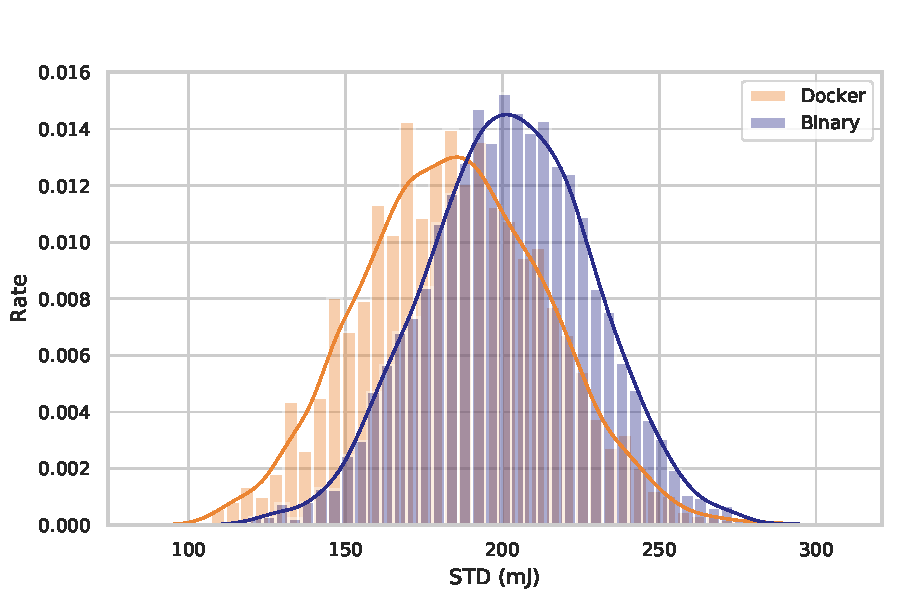
\includegraphics[width=.9\linewidth]{imgs/docvsbin}}
    \caption{Comparing the variation of binary and Docker versions of aggregated \textsf{LU}, \textsf{CG} and \textsf{EP} benchmarks}\label{fig:docker}
\end{figure}